\chapter{Testing}


\section{Introduction}
In our scenario test strategy is used to test the functionality of our system. We have to use to cover all scenarios. Main focus is on Functional Testing. In Functional Testing test case are used to test the application interface.\\
In our system testing is going to be done at individual module level. Each module will be undergone to Unit Testing and expected result is supposed to be same as actual result.\\

% This section type your project contents 

\section{White Box Testing}
White box testing is a security testing method that can be used to validate whether code implementation follows intended design, to validate implemented security functionality, and to uncover exploitable vulnerabilities. White box testing includes analyzing data flow, control flow, information flow, coding practices, and exception and error handling within the system, to test the intended and unintended software
behaviour.\\


% This section type your project contents 

\section{Black Box Testing}
Black box testing takes an external perspective of the test object to derive test cases. These tests can be functional or non-functional, though usually functional. The test designer selects valid and invalid input and determines the correct output. There is no knowledge of the test object’s internal structure.\\



% This section type your project contents 


\section{Validation Testing}
\subsection{Requirements}
\textbullet \hspace{0.2cm} Username must be not blank \\
\textbullet \hspace{0.2cm} Password must be not blank \\
\textbullet \hspace{0.2cm} login with invalid username and valid password\\
\textbullet \hspace{0.2cm} Login with valid username and invalid password\\
\textbullet \hspace{0.2cm} Login with valid credentials \\


\begin{table}[hp]
\centering
\begin{tabular}{|c|c|}
\hline
\textbf{Test Case ID}  & \textbf{Test Case Description} \\
\hline
TC01 &	Login with blank Username \\\hline
TC02 &	Login with blank Password\\\hline
TC03 &	Login with invalid username and valid password \\\hline
TC04 &	Login with valid username and invalid password\\\hline
TC05 &	Login with valid credentials \\\hline

\end{tabular}
\end{table}

% This section type your project contents 

\section{GUI Testing}
The criterion of the user interface is graphical which less time consuming for user but more complexes for the programmer.\\

\pagebreak
\textbf{Test Case 01}
\begin{center}
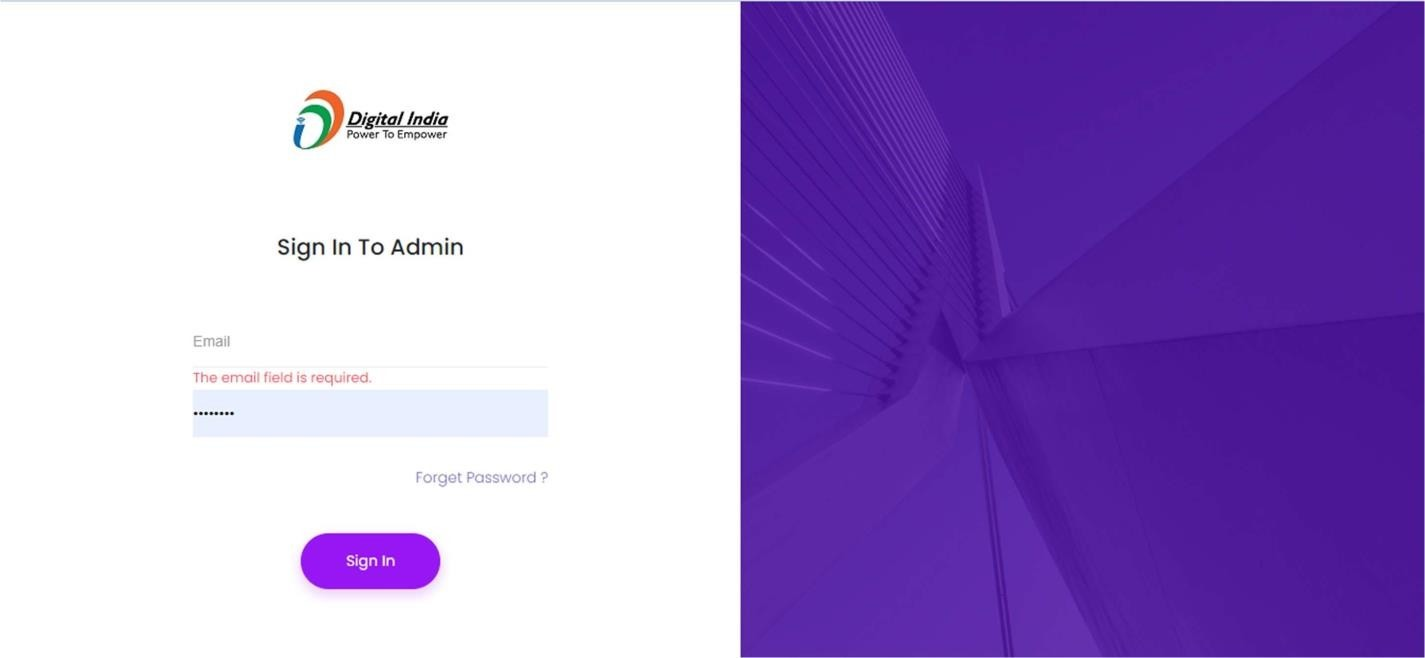
\includegraphics[height=9cm,width=14cm]{Admin/TC01}
\end{center}

\textbf{Test Case 02}
\begin{center}
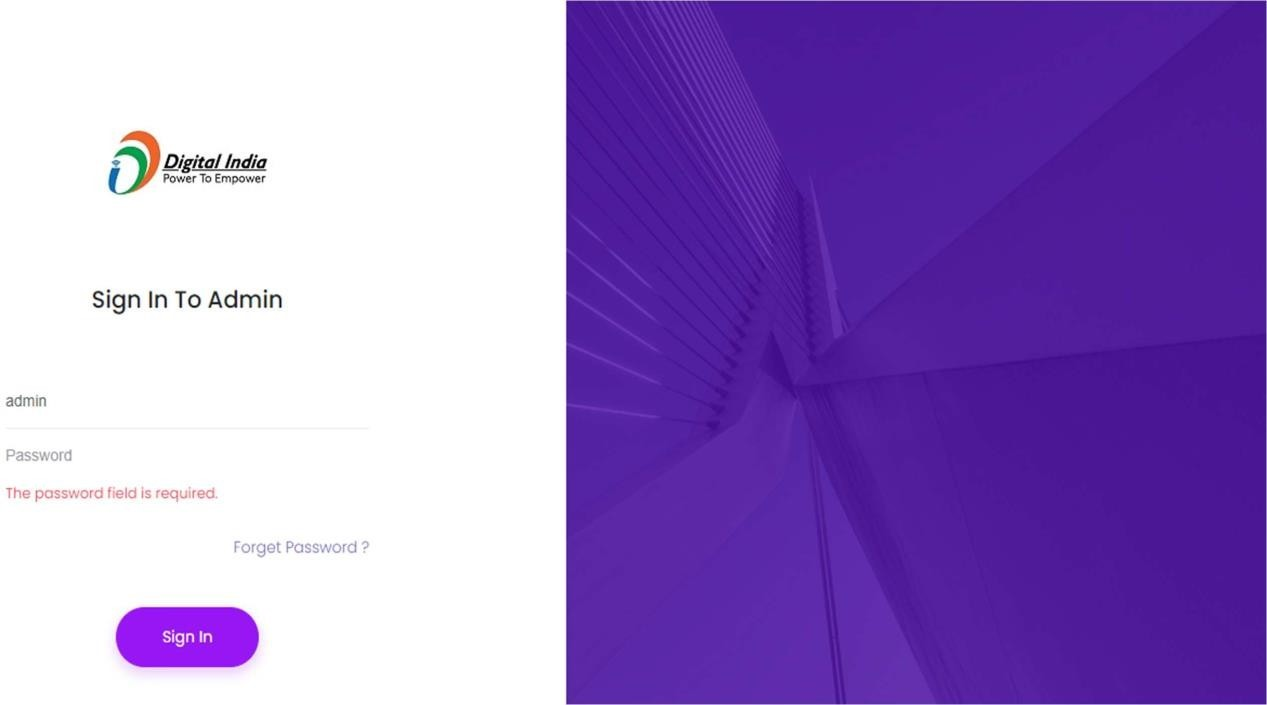
\includegraphics[height=9cm,width=14cm]{Admin/TC02}
\end{center}
\pagebreak

\textbf{Test Case 03}
\begin{center}
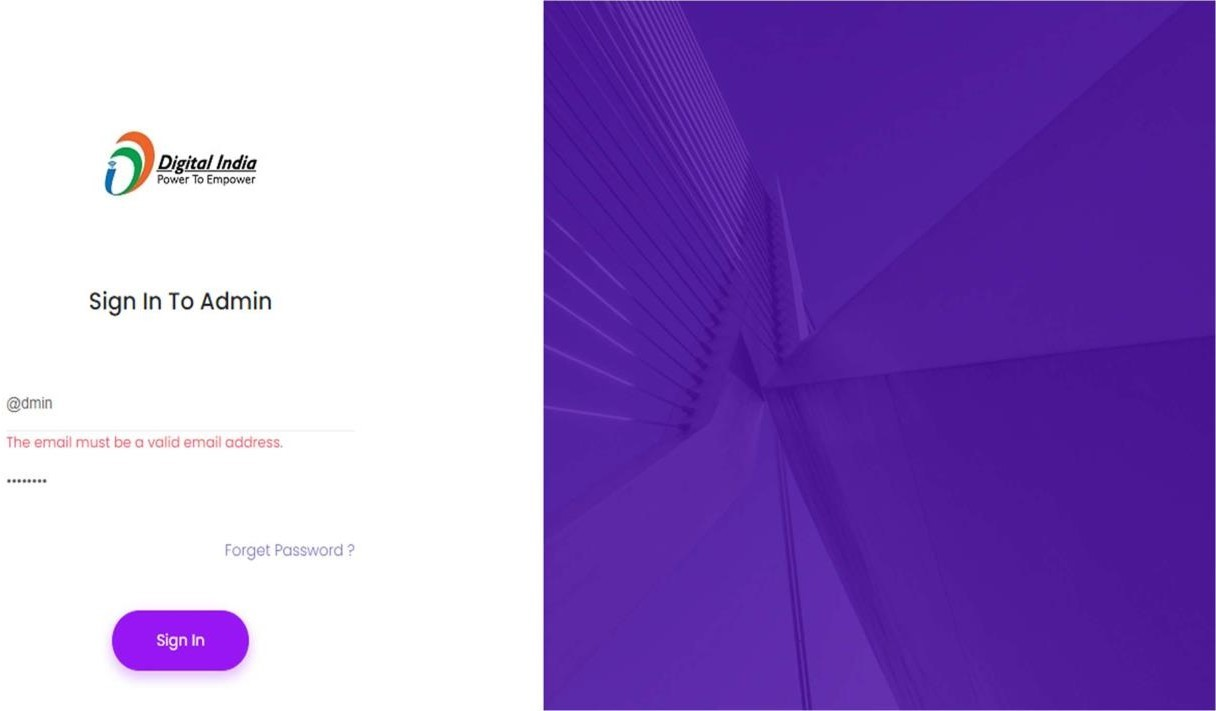
\includegraphics[height=9cm,width=14cm]{Admin/TC03}
\end{center}

\textbf{Test Case 04}
\begin{center}
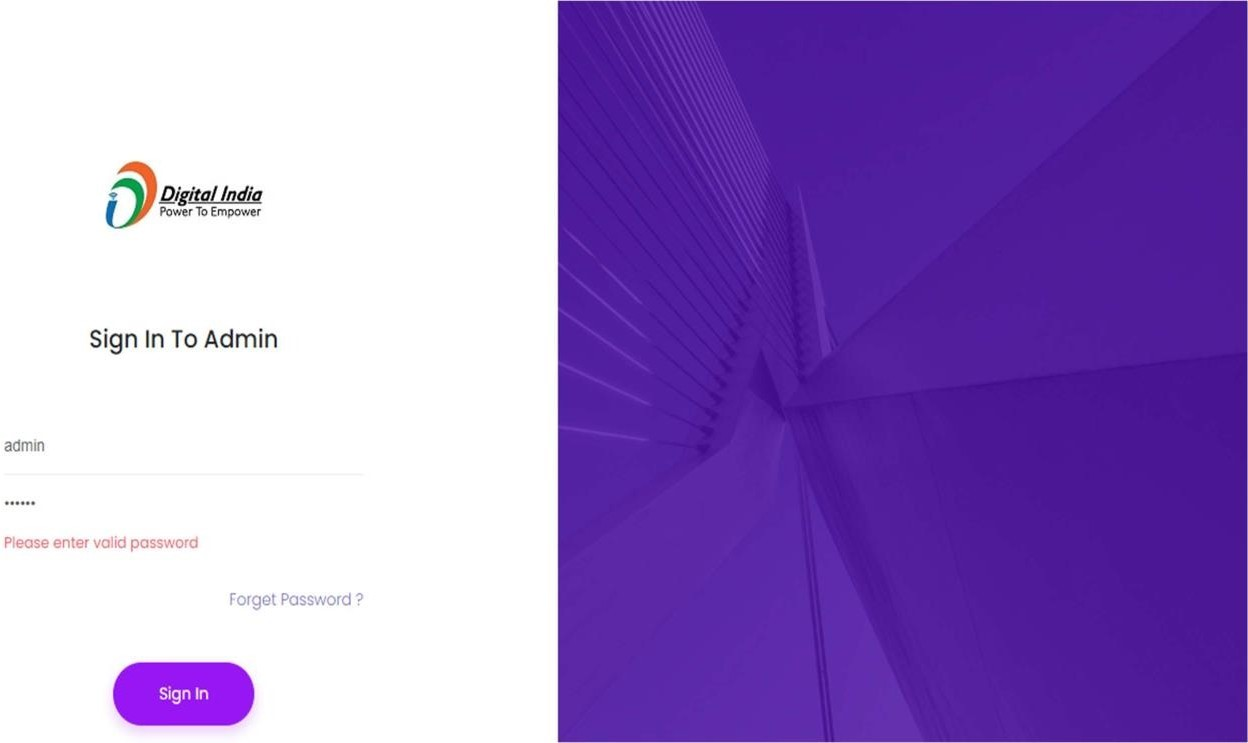
\includegraphics[height=9cm,width=14cm]{Admin/TC04}
\end{center}
\pagebreak

\textbf{Test Case 05}
\begin{center}
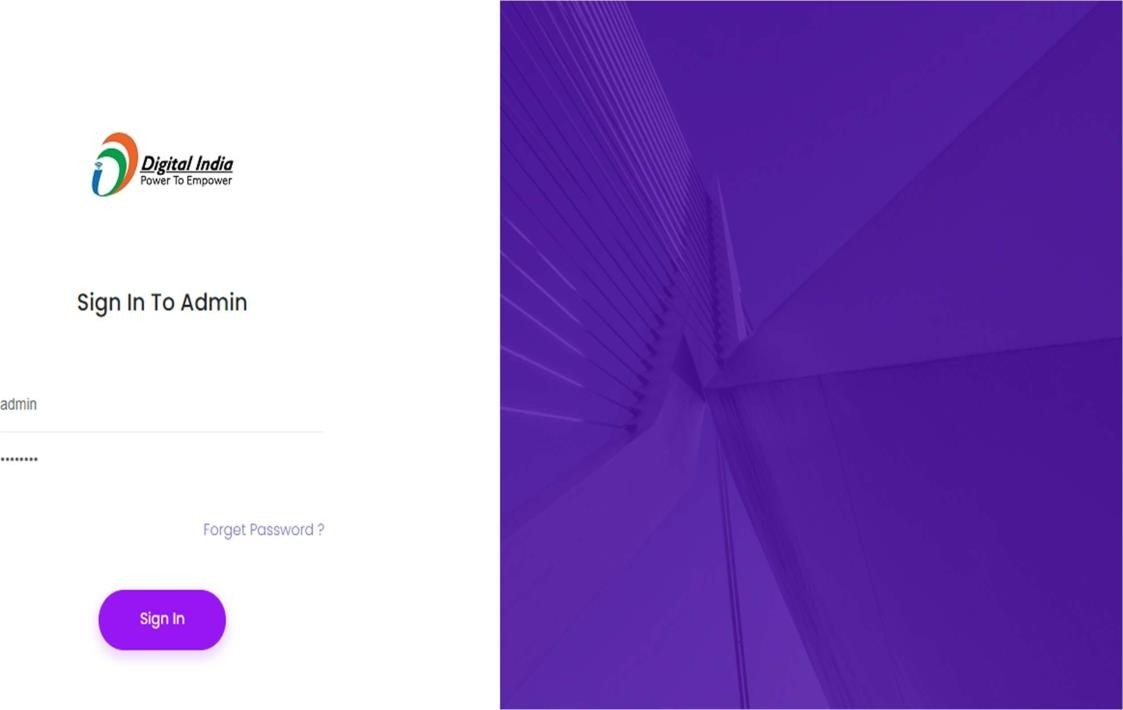
\includegraphics[height=9cm,width=14cm]{Admin/TC05}
\end{center}

% This section type your project contents 